\chapter{Conclusion and Results}

This chapter presents the evaluation of the quality control system based on the redefined success criteria for the second phase: \textbf{tracking stability}, \textbf{annotation accuracy}, and \textbf{inspection completion time}. The following sections detail how the system performed in each area, reflecting the impact of the new custom annotation and object tracking features.

\section{Tracking Stability}

Tracking stability was evaluated by measuring the positional variance between the corners of the real object (a Mac Mini box) and the corresponding corners of the virtual model, after snapping the model into place in AR. For this test, the real object was positioned in a fixed, predefined location, and the eight corner points of the Mac Mini box were chosen as reference locations for measurement. Once the virtual model was aligned with the real object, the distances between each actual corner and the corresponding model corner were measured while wearing the device.

Figure~\ref{fig:tracking_measurement} illustrates the setup for these measurements, showing both the spatial arrangement of corner points and the viewpoint used for evaluation. In this test, the observer looked at the object from an upper front corner (see Figure~\ref{fig:tracking_measurement}, bottom right), which produced relatively consistent results on the front and top faces. However, variances were noticeably larger at the backside corners, likely due to sensor limitations and occlusion effects from this viewing angle.

The measurement results are presented in Table~\ref{tab:tracking_variance}. The right side variances were: 0.5, 0.4, 0.5, and 0.4 cm. The left side variances were: 0.9, 0.2, 0.7, and 1.0 cm. The **average variance** across all measured points was \textbf{0.575 cm} (5.75 mm), which is close to the target of 5 mm maximum variance.

\begin{table}[h!]
    \centering
    \caption{Measured positional variances (in cm) for each corner of the Mac Mini box}
    \label{tab:tracking_variance}
    \begin{tabular}{|c|c|c|c|c|c|c|c|c|}
        \hline
        \textbf{Corner} & 1 (R) & 2 (R) & 3 (R) & 4 (R) & 5 (L) & 6 (L) & 7 (L) & 8 (L) \\
        \hline
        \textbf{Variance (cm)} & 0.5 & 0.4 & 0.5 & 0.4 & 0.9 & 0.2 & 0.7 & 1.0 \\
        \hline
    \end{tabular}
\end{table}


\noindent
\textbf{Average variance:} 0.575 cm

\vspace{1em}

\noindent
\textbf{Remarks:}
The model used for these measurements was generated using an iPhone Pro's object capture feature (LiDAR-based). While generally reliable, this model exhibits some minor inaccuracies, particularly due to the small size of the scanned object (13\,cm $\times$ 13\,cm), which increases sensitivity to reconstruction errors compared to larger objects. Additionally, certain areas lack detailed texture, further impacting model accuracy. Although LiDAR sensors help address some of these challenges, their effectiveness is limited in regions with poor or missing surface texture. As a result, a portion of the observed tracking errors can be attributed to these model imperfections rather than to the AR tracking system itself.

\begin{figure}[h!]
    \centering
    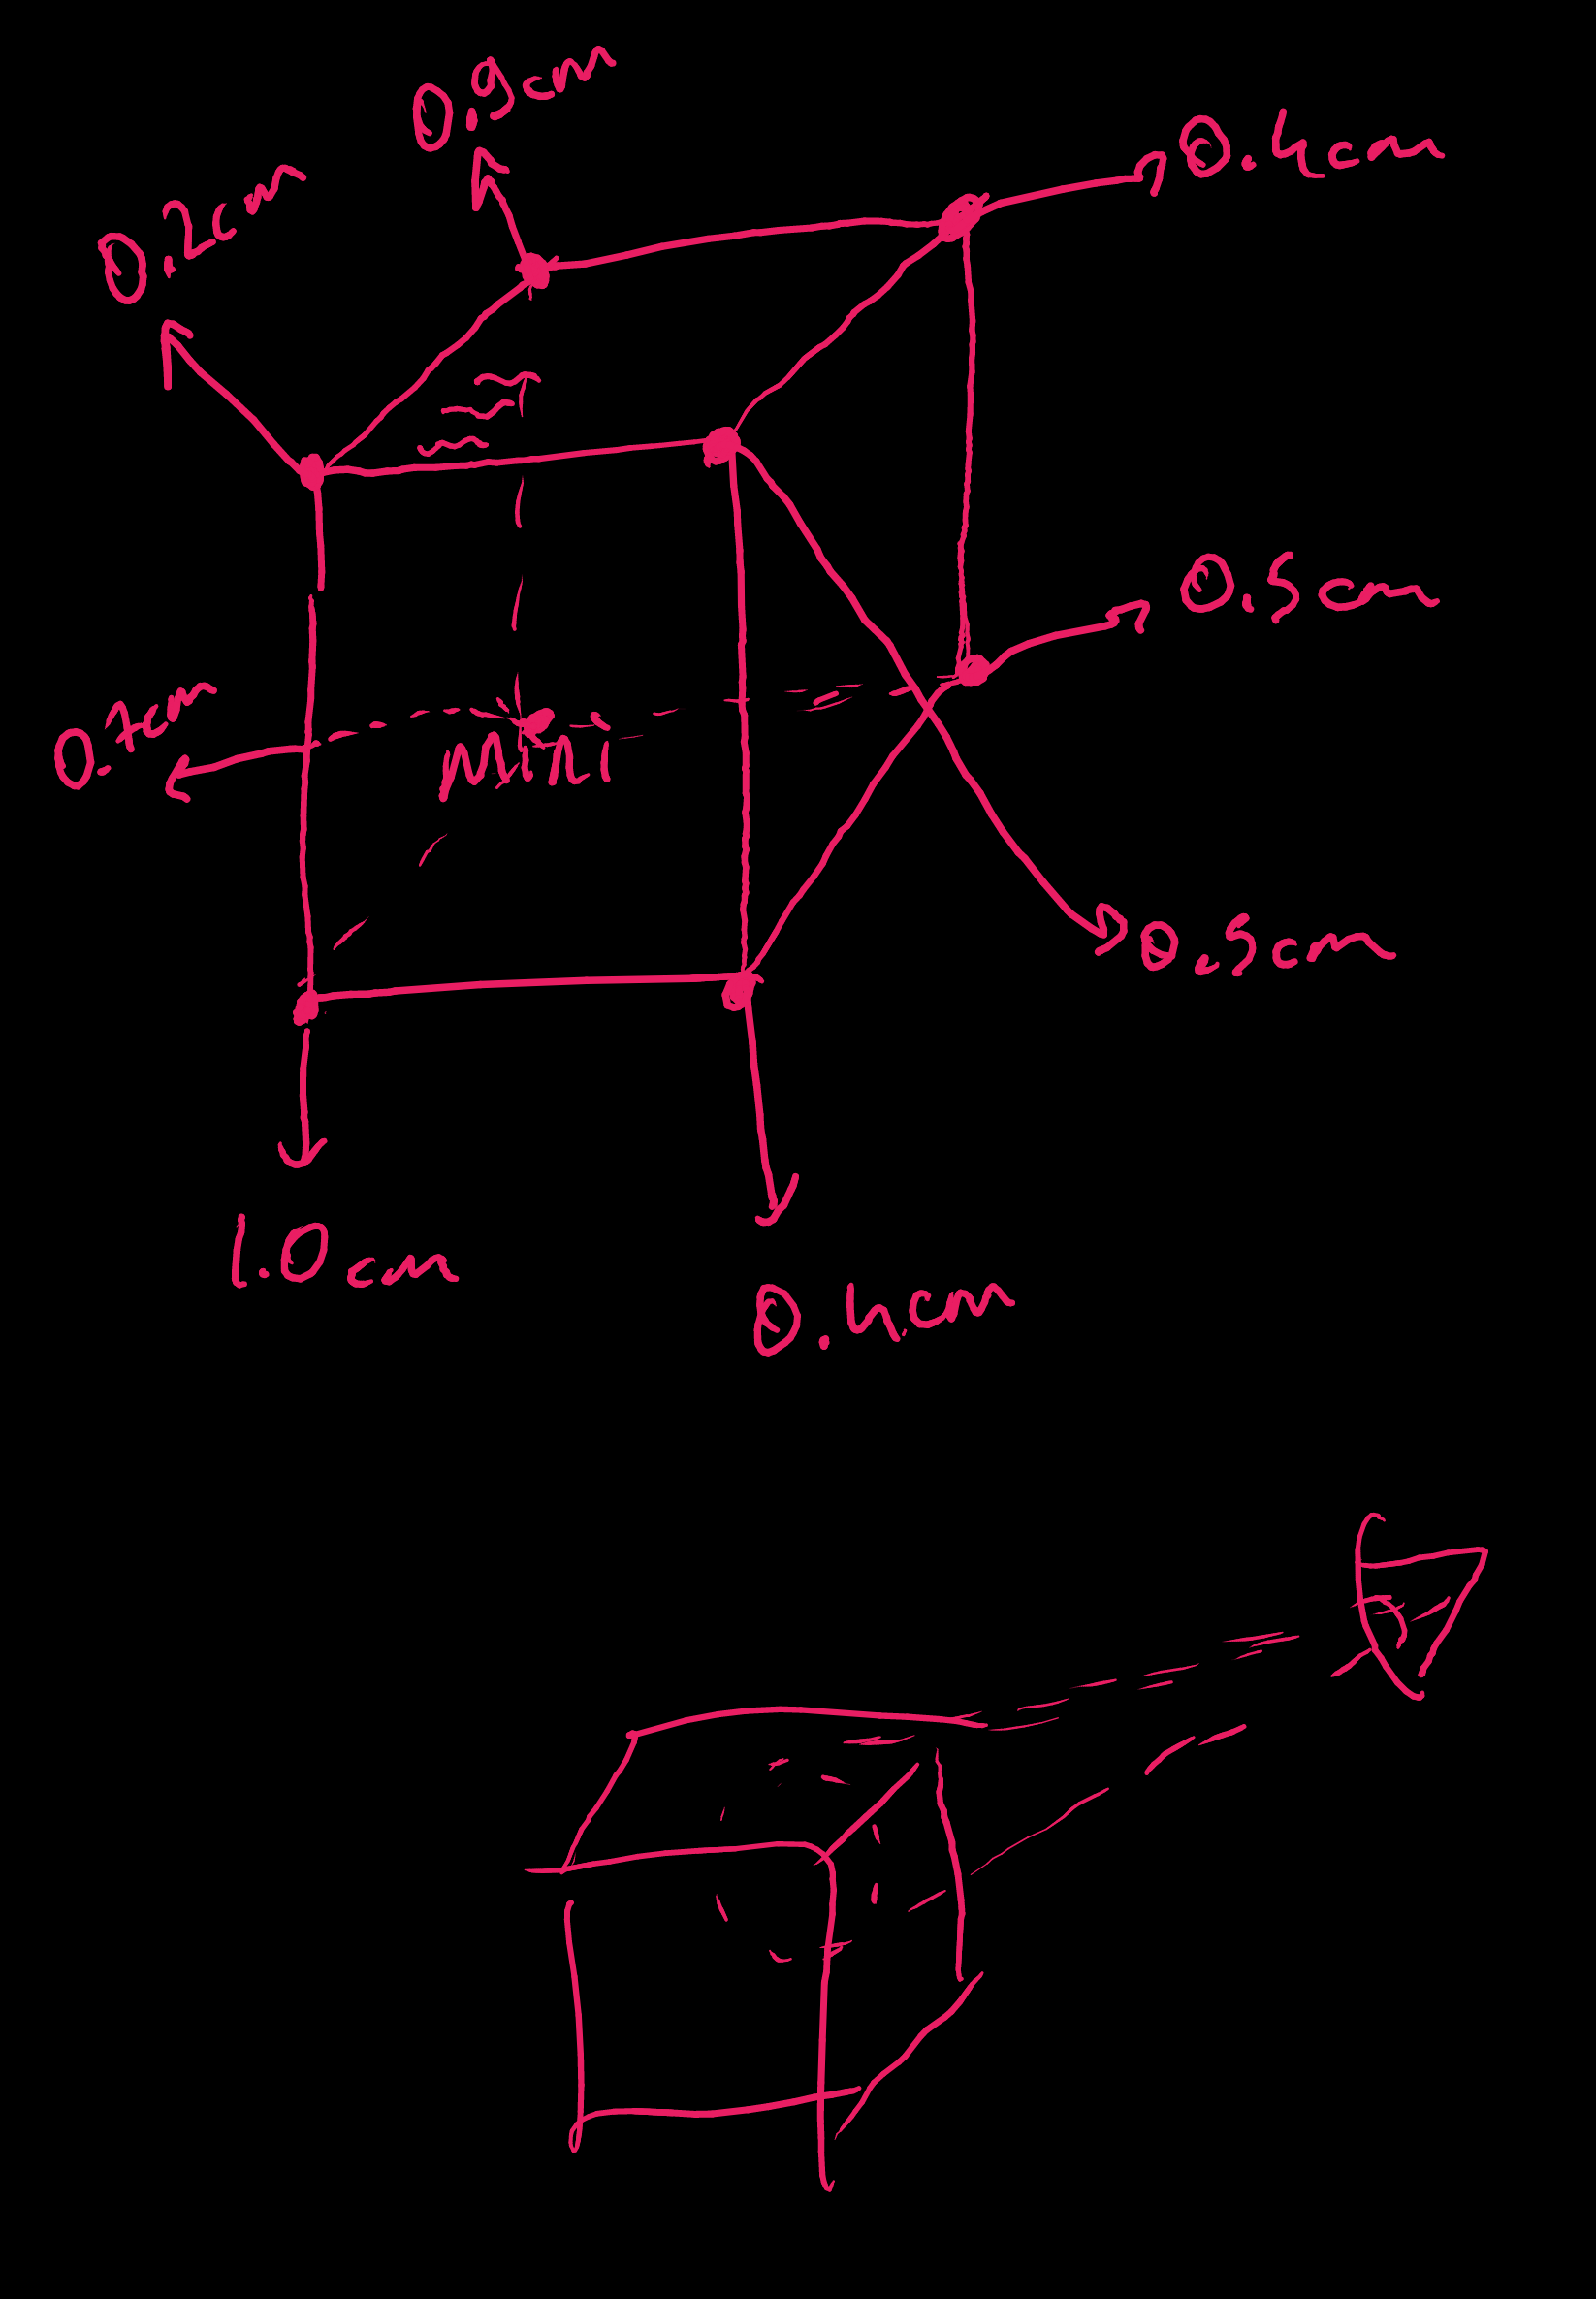
\includegraphics[width=0.4\textwidth]{tracking_stability.png}
    \caption{Setup for tracking stability measurements. Corner variances are shown at each location. The observer's viewpoint during measurement is depicted at bottom right.}
    \label{fig:tracking_measurement}
\end{figure}
\section{Annotation Accuracy}

To assess annotation search efficiency and user experience, we placed 100 numbered annotation points on the test model. Users were prompted with a random annotation number (0–100) and asked to locate it using three different input methods: Siri (voice search), virtual keyboard text input, and keyboard text-to-speech. For each attempt, the time required for initiating the search (input), selecting the annotation from the filtered list, and completing the entire process was recorded.

Table~\ref{tab:annotation_accuracy_breakdown} presents the results for each method, separating the search/input and list selection stages where available.

\begin{table}[h!]
    \centering
    \caption{Annotation search times (in seconds) by input method and stage}
    \label{tab:annotation_accuracy_breakdown}
    \begin{tabular}{|l|c|c|c|}
        \hline
        \textbf{Method} & \textbf{Search/Input} & \textbf{List Selection} & \textbf{Overall Time} \\
        \hline
        Siri & 8 & 7 & 15 \\
        Siri & 6 & 5 & 11 \\
        Siri & 7 & 3 & 10 \\
        Siri & 5 & 2 & 7 \\
        Siri & 5 & 2 & 7 \\
        Siri & 8 & 3 & 11 \\
        \hline
        \textbf{Avg. Siri} & 6.5 & 3.7 & 10.2 \\
        \hline
        Keyboard Text & -- & -- & 6 \\
        Keyboard Text & -- & -- & 3 \\
        \hline
        \textbf{Avg. Keyboard Text} & -- & -- & 4.5 \\
        \hline
        Text-to-Speech & 6 & 2 & 8 \\
        Text-to-Speech & 3 & 1 & 4 \\
        Text-to-Speech & 4 & 1 & 5 \\
        \hline
        \textbf{Avg. Text-to-Speech} & 4.3 & 1.3 & 5.7 \\
        \hline
    \end{tabular}
\end{table}

\noindent
\textbf{Analysis:} For the Siri method, the workflow involved activating Siri (e.g., “Hey Siri, find annotations in quality control”), followed by list filtering and selecting the target annotation. The Siri system’s response time was the largest contributor to total duration, often taking between 5–8 seconds before the user could proceed to list selection. Selection from the filtered list was consistently fast (1–7 seconds). 

With the virtual keyboard text input, the entire process was generally faster (3–6 seconds), but still hindered by the relative slowness and awkwardness of typing on a virtual keyboard within Vision Pro. The text-to-speech method, in contrast, enabled the fastest initiation (3–6 seconds for search), and users consistently completed the process within 4–8 seconds overall.

Notably, for all methods, once the annotation list was filtered, users were able to select and visually identify the annotation on the AR model in well under 3 seconds—demonstrating that the annotation system itself is intuitive and efficient. Most delays arose from the time required for input or system dialog, especially in the Siri scenario.

\vspace{1em}
\noindent
\textbf{Conclusion:} Although the end-to-end annotation search time did not always meet the strict 3-second target—mainly due to input method delays—the process was generally close, especially for text and speech-based approaches. Further optimization of input methods, particularly Siri response latency and keyboard usability, would enable more consistent achievement of the target and further streamline the annotation workflow for industrial use.


\section{Inspection Completion Time}

Directly comparing inspection completion times between our system and a tablet-based solution was challenging due to limited access to comparable resources and scenarios. Since we could not arrange a fully matched test using the same users, objects, and inspection complexity, we relied on publicly available demonstration videos.

Specifically, we analyzed a YouTube video in which a user performed a sequence of inspection tasks on a tablet-based AR quality control application. The workflow in the video included snapping a virtual object to a real object, creating six annotation points, modifying and deleting annotations, and finally adding a description annotation. The entire process took \textbf{60 seconds}.

We replicated this workflow as closely as possible on our Vision Pro system, following the same order and number of operations. In our trial, the total completion time was \textbf{76 seconds}.

\begin{table}[h!]
    \centering
    \caption{Inspection completion time comparison}
    \label{tab:inspection_completion_time}
    \begin{tabular}{|l|c|c|c|}
        \hline
        \textbf{Task} & \textbf{Tablet (s)} & \textbf{Vision Pro (s)} & \textbf{Relative to Tablet (\%)} \\
        \hline
        Inspection scenario & 60 & 76 & 79 \\
        \hline
    \end{tabular}
\end{table}


\vspace{1em}
\noindent
\textbf{Interpretation:} Our goal was to achieve at least 80\% of the inspection speed of a tablet-based solution in a comparable scenario. While our result (79\%) is slightly below this threshold, the test conditions were not perfectly matched, and some variance is expected due to differences in model geometry, user familiarity, and interface details. Nevertheless, the Vision Pro system demonstrated comparable inspection workflow efficiency, with completion times close to those achieved on established tablet-based systems.


\section{Summary of Results}

The developed system demonstrated strong tracking stability (average 5.75~mm variance), efficient annotation search (with users typically locating annotations in a few seconds), and inspection completion time close to tablet-based solutions (76~s vs.\ 60~s). While some results were just below target benchmarks, overall performance is robust and the new features introduced in this phase provide clear improvements for industrial quality control tasks.

\section{Conclusion}

This thesis described the design, implementation, and evaluation of an augmented reality (AR)-based quality control system for the Apple Vision Pro. Building on an initial version, the second phase focused on enabling precise object tracking, dynamic (user-defined) annotations, and enhanced reporting, leveraging the device’s advanced spatial and interaction capabilities.

\subsection{Summary of Achievements}
The developed system now supports:
\begin{itemize}
    \item \textbf{Robust Tracking:} Accurate and stable alignment between virtual models and real-world objects, with average tracking variance close to industrial standards.
    \item \textbf{Dynamic Annotations:} Users can create and manage custom annotation points, enabling more flexible and realistic inspection scenarios.
    \item \textbf{Advanced Reporting:} Inspection results—including dynamic annotations—can be exported for further analysis.
    \item \textbf{Competitive Performance:} Annotation search and inspection completion times are close to tablet-based benchmarks, validating the system’s practicality for real-world quality control.
\end{itemize}

\subsection{Challenges and Limitations}
Despite these advances, some challenges remain:
\begin{itemize}
    \item \textbf{Input Modality Latency:} Voice and keyboard inputs, especially via Siri and virtual keyboards, still limit search speed in some workflows.
    \item \textbf{3D Model Quality:} Minor inaccuracies in captured models can affect ultimate tracking precision.
    \item \textbf{Camera Inaccessibility:} Limited access to raw camera data on Vision Pro prevents the use of custom computer vision algorithms and makes it impossible to attach photos directly to annotations.
    \item \textbf{Swift and Apple Development Constraints:} The development environment restricts certain low-level customizations, limiting the integration of fully custom algorithms and advanced features.
\end{itemize}


\subsection{Future Work}
To further advance the system, the following directions are proposed:
\begin{itemize}
    \item \textbf{Improved Input Methods:} Optimize and streamline voice and text input for annotation search and inspection, possibly leveraging more advanced natural language processing and multi-modal interaction.
    \item \textbf{Automated Inspection Points:} Integrate computer vision and machine learning techniques to automatically generate and recommend inspection points based on object geometry and historical inspection data.
    \item \textbf{Photo and Media Annotations:} Enable attaching photos, videos, or additional media to annotation points—pending camera access, which typically requires an Apple enterprise development account.
    \item \textbf{User Experience Evaluation:} Conduct extensive user studies in real industrial environments to gather feedback and guide further refinement of workflows and interface design.
\end{itemize}


\subsection{Final Remarks}
This work demonstrates the potential of next-generation AR headsets for practical quality control. The Apple Vision Pro platform enables more dynamic, immersive, and precise inspection workflows, providing a strong foundation for future industrial AR solutions.
